%!TEX root=paper.tex
\section{Method}\label{sec:method}

We consider first approaches which can effectively reorder the sequence of regions to maximize the chance that correct detections will be found, based on inference from relatively lightweight features.  We show that basic strategies, such as simply randomly reordering the boxes such that they do not have a degenerate spatial layout, provides a surprising boost, and that very simple features such as region and gradient statistics can provide some signal that is useful to prioritize regions, but that those are relatively weak.

Features based on convolutional mid-level primitives are more powerful, as they are directly related to our final detector.  We consider approximate measures computed from a grid of mid-level features; this proves to be a powerful signal, and provides a clear boost when the time required to compute that feature is not considered.    But even with a fast image pyramid to compute them globally for all regions, the time required is unfortunately large enough to significantly dilute their impact.

What is thus desired is a method which can compute an early feature which indicates the region priority, and then can use that same feature in the subsequent classification, with minimal computation that cannot be so amortized.  We formulate a cascade version of the RCNN architecture which has these desirable properties, and show that either alone or in concert with other methods below, it can effectively learn a ``Timely'' approach to the detection computation.

We first review the base model that our work is derived from, the R-CNN method, in the following subsection.  We then present our approach to region prioritization using simple features based on basic region and gradient properties in \autoref{sec:region} and \autoref{sec:gradient}.  We then consider mid-level features in \autoref{sec:dense}, based on a Pyramid scheme which amortizes the computation across overlapping regions, but does not use them for the subsequent computation.  Finally, we present our final model, the Cascade-CNN, in \autoref{sec:ccnn} which combines elements of all of these approaches into a unified scheme: it can prioritize based on low-level features early in the CNN, or expoit more costly mid-level features, and when it has decided to carry the computation to the final detection it does so effectively re-using the computation from the earlier tests, and therefore does not waste additional time.

\subsection{Base model}

We take the Region-CNN (R-CNN) \cite{Girshick-CVPR-2014} method as our point of departure.
As summarized in \autoref{fig:rcnn}, R-CNN starts with external region-of-interest proposals (ROIs).
ROIs are taken in batches: transformed to canonical size, and classified with a CNN, obtaining multi-class scores for each region.
After all batches have been scored, ROIs are post-processed with non-maximal suppression and other bounding box refinement to obtain the final detections.

We start with the same ROI proposals, but first score all proposals with a quick-to-compute feature.
We then select a batch of highly-scoring ROIs and classify them with the CNN -- which can additionally be sped up with cascaded structure.
After the batch is scored, we optionally re-score the remaining ROIs, and repeat the process until we're either out of time, or out of regions.
\autoref{fig:combined} summarizes the process.

As shown in \autoref{fig:combined}, the quick-to-compute features are used to select batches of regions in a way that orders the regions most likely to contain ground truth objects earlier than other regions.
This process of region selection does not reject regions flat out, but reorders them to be processed later.

We first tried to simply sort the regions by score and take batches in that sorted order.
Surprisingly, this naive method results in poor performance, and in fact can be worse than taking regions in an entirely random order.
We hypothesize that this is because the highest scoring regions may all be overlapping with each other, and only result in one detection after non-maximal suppression and other post-processing of detections.
Guided by this intuition, we consider a more dynamic approach to region selection:
we put regions in a random order, set a threshold such that only half of the unexamined regions score above it, take a batch of the above-threshold regions in their order, update the threshold, and repeat.

\begin{figure}[h!]
\begin{center}
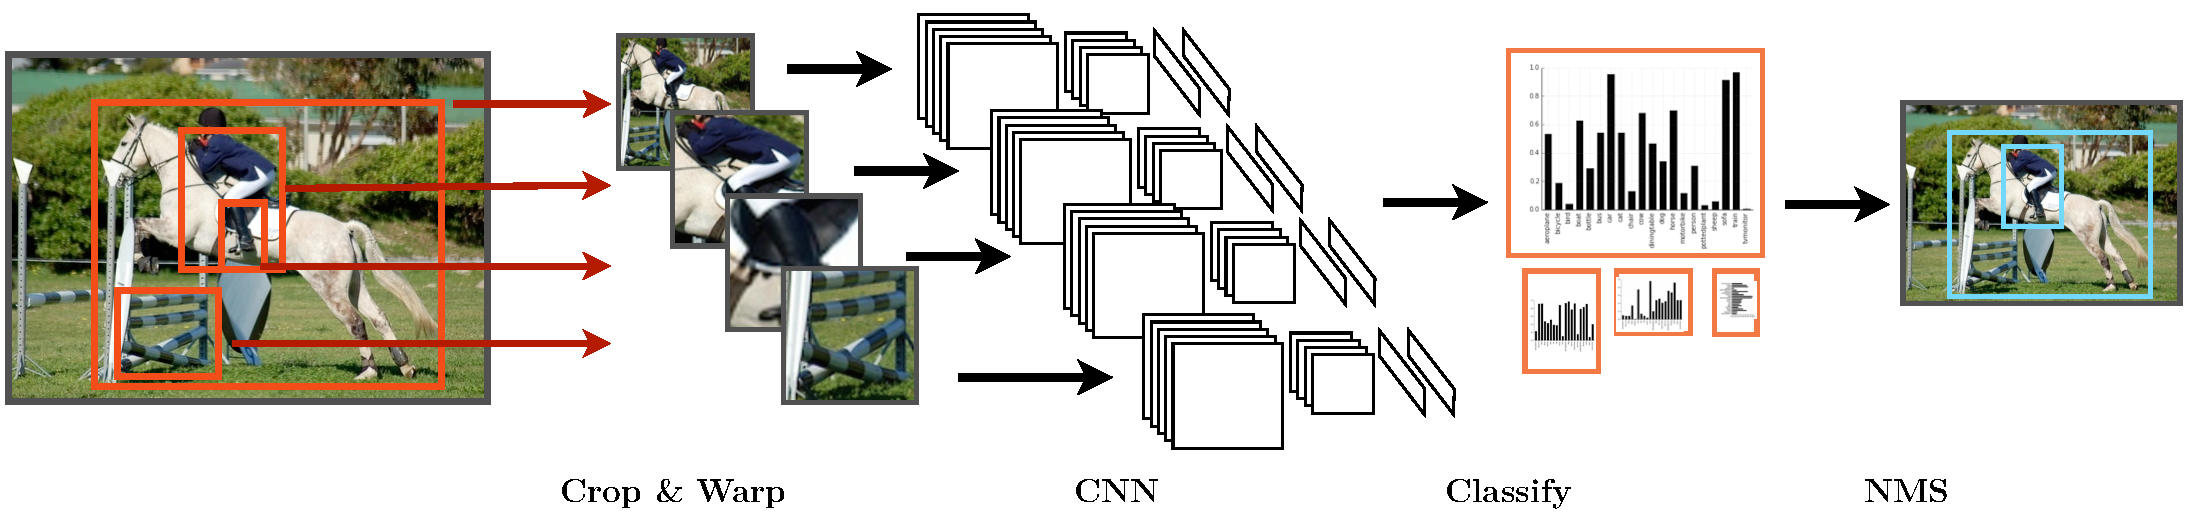
\includegraphics[width=0.98\columnwidth]{figures/rcnn.pdf}
\caption{
R-CNN architecture: image regions are cropped, resized, and each one fed through a CNN with classification layers.
The classifier outputs are post-processed to give the final detections.
}\label{fig:rcnn}
\end{center}
\end{figure}

\begin{figure}[h!]
\begin{center}
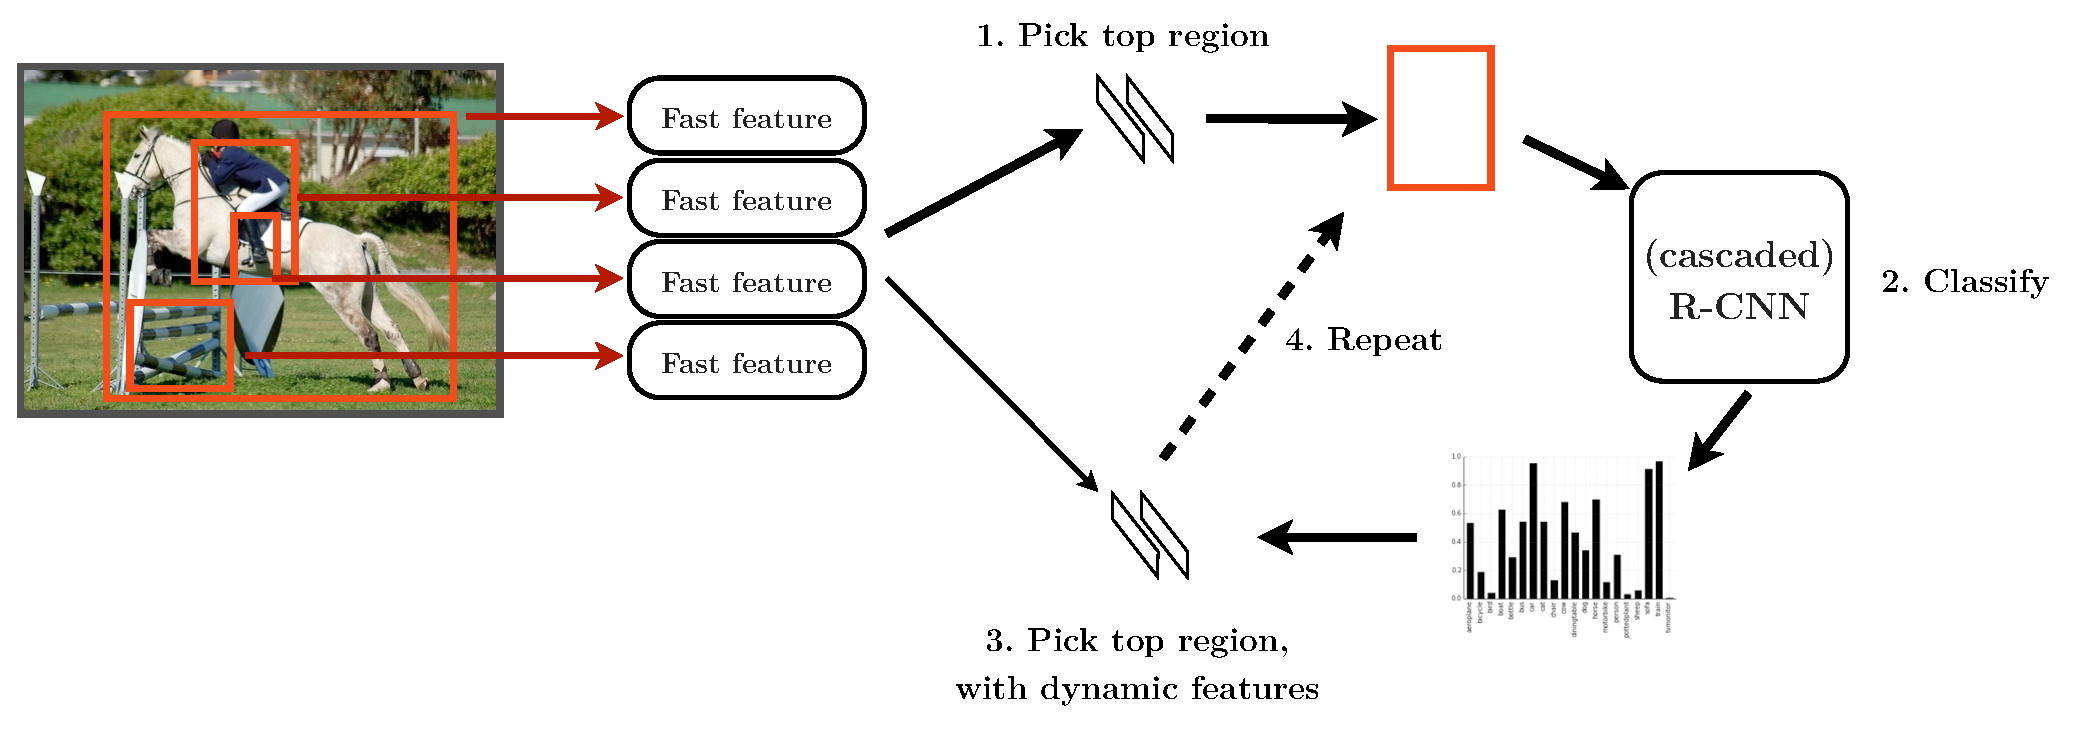
\includegraphics[width=0.98\columnwidth]{figures/combined.pdf}
\caption{
Our method scores each region of interest with a fast feature (we evaluate several), allowing us to pick promising regions first.
The regions are classified with the original CNN, or a sped-up Cascade-CNN.
The properties of the regions can play a role in selecting the next batch of regions.
}\label{fig:combined}
\end{center}
\end{figure}

%%%%%%%%%%%%%%%%%%%%%%%%%%%%%%%%%%%%%%%%%%%%%%%%%%%%%%%%%%%%%%%%%%%%%%%%%%%%%%%
\subsection{Region statistics}\label{sec:region}
For the quick-to-compute feature, we consider statistics about ROI location and overlap with other regions.
We compute a very simple feature for each ROI: its normalized location,
its scale($\sqrt{\text{width} \times \text{height}}$),
aspect ratio ($\log \sqrt{\text{width} / \text{height}}$),
and normalized counts of overlapping regions, at different PASCAL overlap thresholds (0, 0.2, 0.6).

This simple feature works suprisingly well for filtering regions to process first, and is always included in concatenation with the more complex features that are described next.

%%%%%%%%%%%%%%%%%%%%%%%%%%%%%%%%%%%%%%%%%%%%%%%%%%%%%%%%%%%%%%%%%%%%%%%%%%%%%%%
\subsection{CNN pixel gradient computation}\label{sec:gradient}

One fast-to-compute feature we consider for the preliminary featurization of ROIs is the pixel gradient, back-propagated throgh the classifier CNN applied to the whole image.
This gradient corresponds to a kind of saliency map onto the image \cite{Simonyan-ICLR-2014}, and can therefore be used to evaluate ROIs.

We have fine-tuned an ``AlexNet'' \cite{Krizhevsky-NIPS-2012} CNN using the PASCAL VOC 2007 classification challenge.
Unlike the ILSVRC, the PASCAL VOC is a multi-label prediction task, with at times multiple correct labels for an image.
Accordingly, we implement a cross-entropy loss layer to train a simple multi-label classifier with binary vector.

This pixel-wise gradient can be seen as a first-order approximation to the weight of a pixel in the classification output.
To compute it, we first run the CNN forward from image input to the prediction layer.
Back-propagating through the model and a last backward pass to the input gives the pixel-wise gradient.
A couple of example images are shown in \autoref{fig:gradient}.

We compute an integral image on this pixel gradient map, allowing near-instant computation of sums in arbitrary regions.
For each region to be evaluated, we compute the total gradient sum, sums for each of the corners, and proportions of in-region vs. out-of-region sums.


%%%%%%%%%%%%%%%%%%%%%%%%%%%%%%%%%%%%%%%%%%%%%%%%%%%%%%%%%%%%%%%%%%%%%%%%%%%%%%%
\subsection{Pyramid amortized R-CNN}\label{sec:dense}

Another fast ROI featurization we consider is a variant of R-CNN that processes the whole image, at multiple scales, with the CNN up to the topmost non-fully-connected layer.
We call this multiscale CNN output a ``feature pyramid''.
As \autoref{fig:dense_rcnn} shows, ROIs are then cropped from the feature pyramid at the best matching scale, warped to a canonical size, and classified.
ROIs are highly overlapping, but their featurization is shared through the pyramid, amortizing its construction cost.
This doesn't work as well as the original R-CNN system, but is much faster, and can therefore be used as the fast feature for the dynamic region selection.

% \subsubsection{Design choices}

We explored a variety of choices while designing Pyramid R-CNN.
We tried using a single scale or a pyramid with 7 levels each separated by a scale factor of $2^{-1/2}$.
For warping, we experimented with canonical sizes of $s \times s$, for $s \in \{5,6,7\}$ and resampling with nearest neighbor or bilinear interpolation.
We also tried two variants of the feature pyramid: the raw feature pyramid or one where each level is max pooled with a $3 \times 3$ pooling window run at a stride of $1$ (to avoid subsampling).

\autoref{tab:prcnn} shows mAP performance on PASCAL VOC 2007 test for these various choices.
The best configuration, in terms of mAP, uses a 7 level pyramid, a warp size of $7 \times 7$ with bilinear interpolation, and max pooling.
The first level of our pyramid is computed from a $1713 \times 1713$ pixel image, which yields a $108 \times 108$ cell feature map.
The gold standard (non-pyramid) R-CNN performance using the same non-fine-tuned CNN is 44.2\% mAP.
Our best result with Pyramid R-CNN is slightly worse, at 41.9\%.

To map a ROI $R$ into the pyramid, we start by computing an ``optimal'' scale defined by $\alpha^* = 227/\min(h,w)$, where $h$ and $w$ are image height and width of $R$.
We then find the nearest level in the pyramid: $l^* = \textrm{argmin}_l |\log(\alpha_l) - \log(\alpha^*)|$, where $\alpha_l$ is the scale factor for pyramid level $l$.
This procedure approximates the scale that R-CNN would use, since it operates on $227$ pixel inputs.

\begin{table}[ht]
\centering
\caption{
    Pyramid R-CNN design choices, vs mAP performance.
    We additionally show two best and two worst performing classes.
}\label{tab:prcnn}
\small{
\begin{tabular}{@{}rccccl@{}}
\toprule
settings      & \mcell{warp 7x7\\nearest}  & \mcell{warp 7x7\\nearest}  & \mcell{warp 7x7\\bilinear}  & \mcell{max pooled 3x3\\warp 7x7\\bilinear} \\
scales        & 1                          & 7                           & 7                          & 7 \\
\midrule
aeroplane     & 31.7                       & 46.8                        & 44.5                       & 47.0 \\
bicycle       & 36.1                       & 50.1                        & 52.6                       & 57.9 \\
bird          & 12.3                       & 25.4                        & 26.7                       & 31.1 \\
boat          & 12.5                       & 20.4                        & 25.7                       & 27.5 \\
bottle        & 11.4                       & 12.9                        & 12.6                       & 19.8 \\
bus           & 17.1                       & 43.6                        & 45.4                       & 50.7 \\
car           & 39.8                       & 54.3                        & 56.7                       & 60.0 \\
cat           & 7.0                        & 39.0                        & 42.4                       & 48.2 \\
chair         & 6.7                        & 11.7                        & 11.8                       & 16.0 \\
cow           & 25.8                       & 41.9                        & 44.1                       & 50.1 \\
diningtable   & 10.2                       & 29.2                        & 33.0                       & 38.6 \\
dog           & 7.2                        & 35.3                        & 36.0                       & 41.6 \\
horse         & 17.3                       & 46.3                        & 51.2                       & 55.8 \\
motorbike     & 27.8                       & 49.4                        & 53.3                       & 56.6 \\
person        & 16.6                       & 28.8                        & 31.3                       & 36.4 \\
pottedplant   & 11.4                       & 17.1                        & 18.6                       & 20.9 \\
sheep         & 19.3                       & 34.4                        & 35.8                       & 40.2 \\
sofa          & 10.3                       & 22.8                        & 29.3                       & 35.8 \\
train         & 17.9                       & 38.1                        & 43.0                       & 44.9 \\
tvmonitor     & 36.3                       & 50.0                        & 54.0                       & 59.7 \\
\midrule
mAP           & 18.7                       & 34.9                        & 37.4                       & 41.9 \\
\bottomrule
\end{tabular}

}
\end{table}

\begin{figure}[h!]
\begin{center}
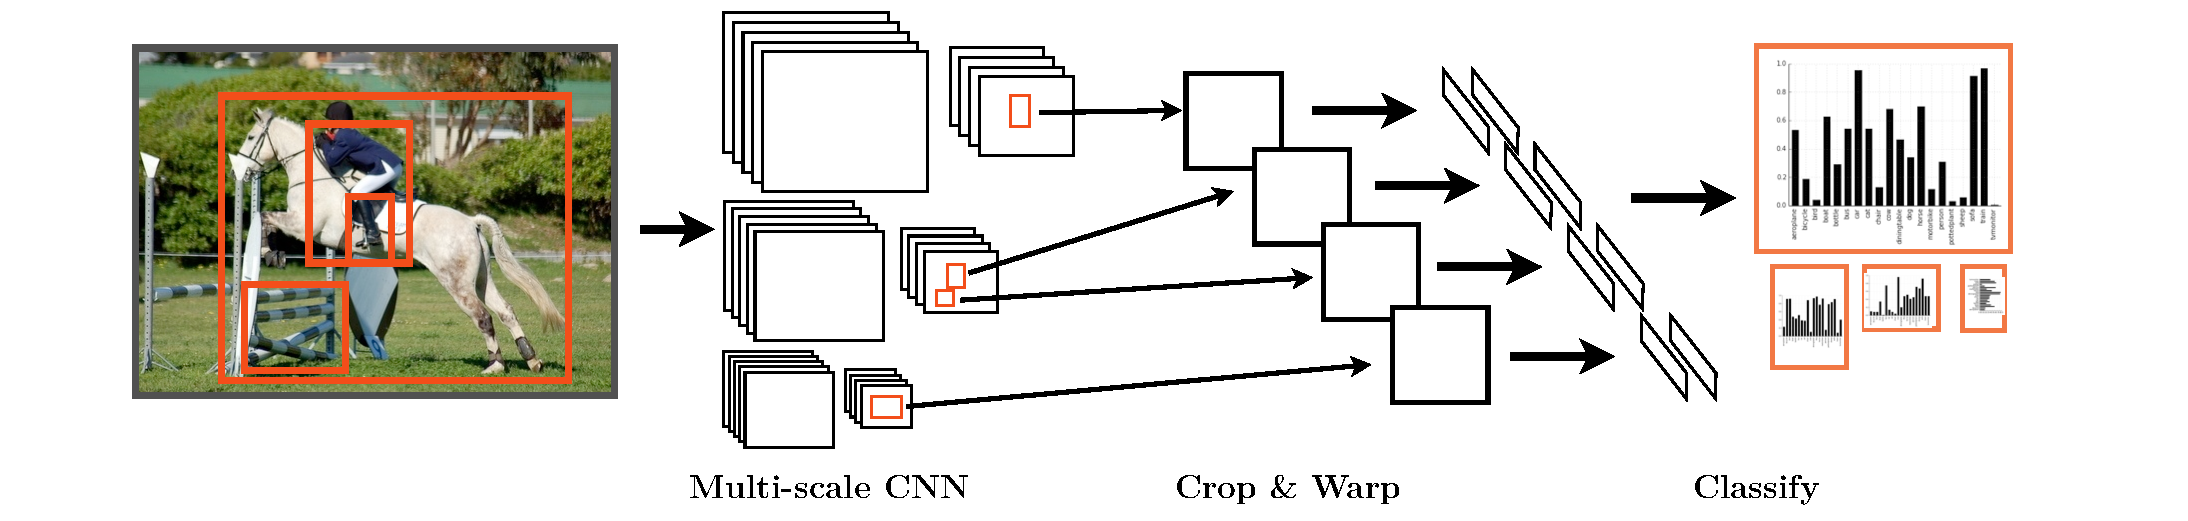
\includegraphics[width=0.98\columnwidth]{figures/dense_rcnn.pdf}
\caption{
Post R-CNN architecture: the whole image is fed through a CNN up to the highest pooling layer.
Regions are cropped from that layer at the best matching scale, resized, and classified.
}\label{fig:dense_rcnn}
\end{center}
\end{figure}

\subsection{Cascaded CNN}\label{sec:ccnn}

Most ROIs that go through the CNN in R-CNN do not contain objects of interest, and are simply background.
It would be useful to quickly reject these regions, without expending the full amount of computation on them. Since most of the time is spend in the convolution layers, we introduce a reject layer after layer 1, 2, and 3, this allows skipping the computation of the following convolutions. These reject layers were trained using the corresponding fine-tuned CNN.

The Cascaded CNN, shown in \autoref{fig:ccnn}, augments the CNN network with an ``Early Reject'' option: after some layers, the network decides whether to keep computing the input with the next layer, or to reject the region since it is background.
For our purpose, the reject layers are trained to separate Background/Foreground, terminating if they are confident that the input is Background. The last classification layer still outputs the full multi-class scores for the surviving regions.

To set the thresholds we took a sample of 140K regions from the images in the validation set containing positive and negative examples. Then we set the threshold for the rejector after first layer to have 0.8 recall on the positive regions. Similarly we set the threshold in for the rejector after the second layer, using the regions that pass the first rejector, to maintain a 0.8 recall on positive regions. And finally we set the threshold for the rejector after the third layer, using the regions that pass the first two rejectors, to maintain a 0.8 recall on positive regions. After every rejection layer the precision on positive regions increase, going from 0.38 to 0.74, while maintaining a recall of 0.8.

To estimate the saving on time by using the rejectors we timed the time spend to process 1000 regions (10 batches or 100) and the time expended in each of the first 3 layers:

\begin{itemize}
\item 1700 ms to process all the layers
\item 270 ms (15\%) in layer 1 (This includes \texttt{conv1}, \texttt{relu1}, \texttt{pool1}, \texttt{norm1})
\item 360 ms (20\%) in layer 2 (This includes \texttt{conv2}, \texttt{relu2}, \texttt{pool2}, \texttt{norm2})
\item 285 ms (15\%) in layer 3 (This includes \texttt{conv3}, \texttt{relu3})
\end{itemize}

Therefore the expected ``lifetimes'' of regions rejected after layer 1, layer 2, layer 3 and those not rejected are  0.15, 0.35, 0.5, 1.0 of the total time taken per region (~1.7 ms).

At test time, we observe how many regions out of the batch size of 100 survive each round of thresholding, and then have a weighted average of a region lifetime in that batch. We multiply the standard batch time of 500ms by that average region lifetime to arrive at the batch time of the cascaded CNN.

\begin{figure}[h!]
\begin{center}
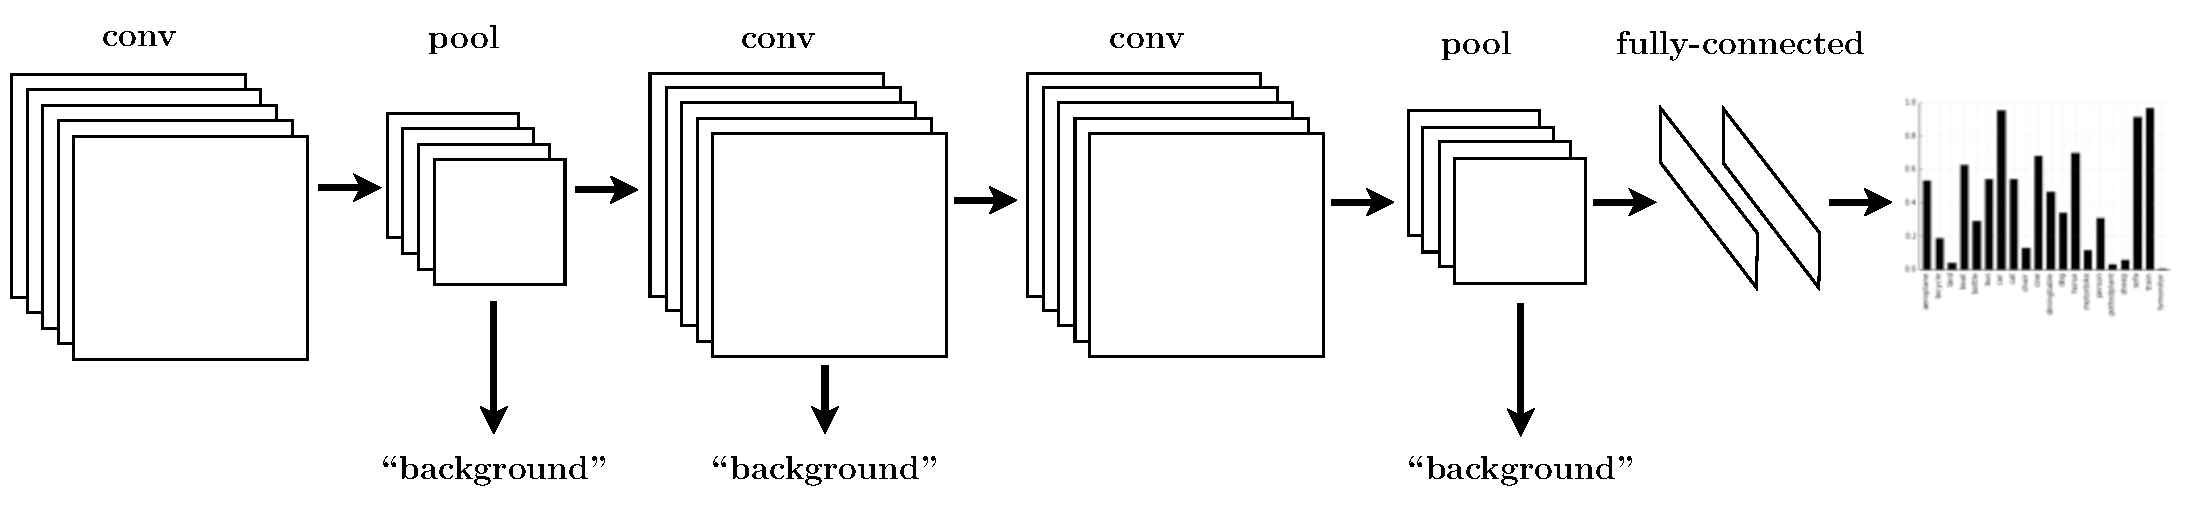
\includegraphics[width=0.98\columnwidth]{figures/ccnn.pdf}
\caption{
The Cascaded CNN has a reject option after pool1, pool2 and conv3 layers.
}\label{fig:ccnn}
\end{center}
\end{figure}
